\subsubsection{Character Buffer}

The character buffer for the video-out port is stored in on-chip memory in the FPGA
on the \DEBoard~board. As illustrated in Figure \ref{fig:chars}$a$, the buffer provides 
a resolution of 80 $\times$ 60 characters, where each character occupies an 8 $\times$ 8
block of pixels on the screen. Characters are stored in each of the locations shown in
Figure \ref{fig:chars}$a$ using their ASCII codes; when these character codes are 
displayed on the monitor, the character buffer automatically generates the
corresponding pattern of pixels for each character using a built-in font. 
Part $b$ of Figure \ref{fig:chars} shows that characters are addressed in the memory by 
using the combination of a {\it base} address, which has the value 
{\sf 0x\baseAddressOffset 9000000}, and an {\it x,y}
offset. Using this scheme, the character at location 0,0 has the address
{\sf 0x\baseAddressOffset 9000000}, 
the character 1,0 has the address {\it base} $+$ (000000 0000001)$_2$ = {\sf 0x\baseAddressOffset 9000001}, 
the character 0,1 has the address {\it base} $+$ (000001 0000000)$_2$ = {\sf 0x\baseAddressOffset 9000080}, and 
the character at location 79,59 has the address {\it base} $+$ (111011 1001111)$_2$ = 
{\sf 0x\baseAddressOffset 9001DCF}. 

\begin{figure}[h!]
   \begin{center}
       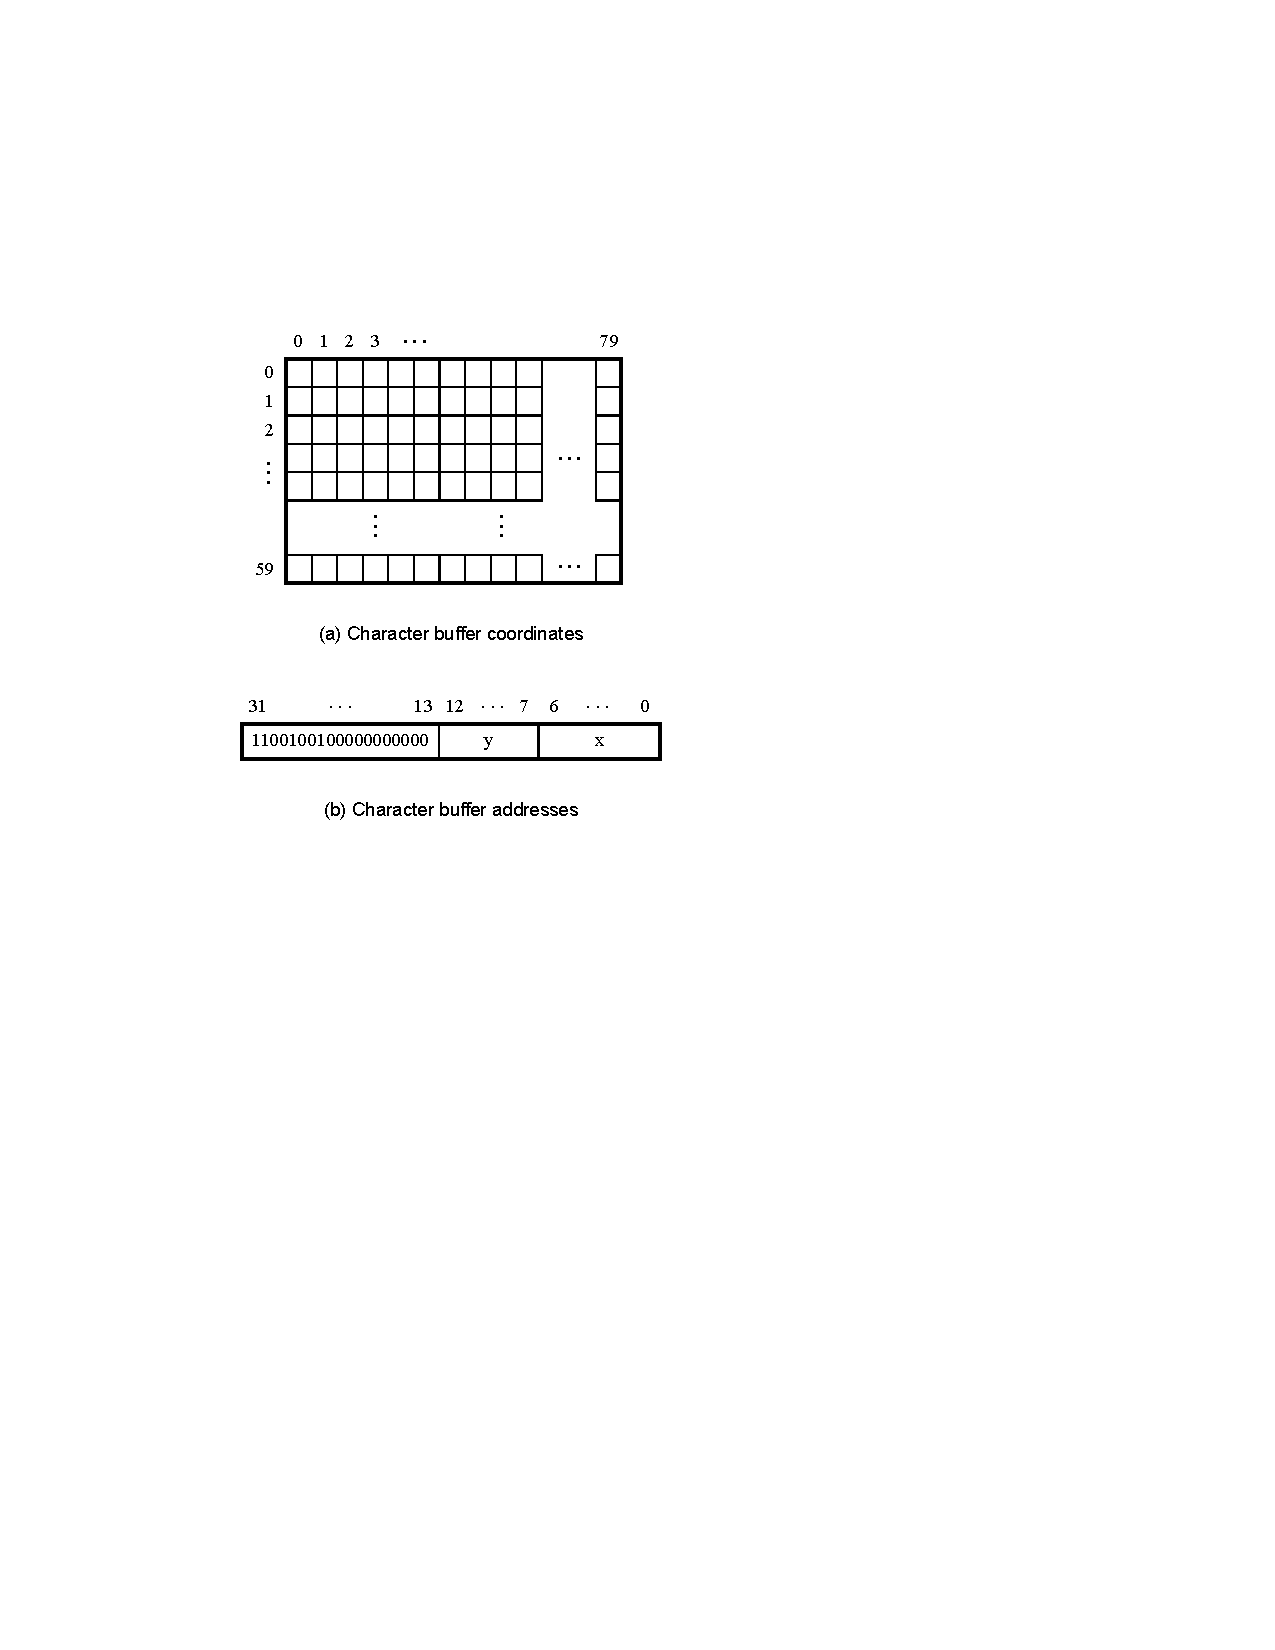
\includegraphics{../../../common/figs/Media_FPGA_Video_Chars.pdf}
   \end{center}
   \caption{Character buffer coordinates and addresses.}
	\label{fig:chars}
\end{figure}
